\documentclass{article}
\usepackage[utf8]{inputenc}
\usepackage[T1]{fontenc}
\usepackage{authblk}
\usepackage{setspace}
\usepackage[margin=1.25in]{geometry}
\usepackage{graphicx}
\graphicspath{ {./figures/} }
\usepackage{subcaption}
\usepackage{amsmath}
\usepackage{amssymb}
\usepackage{booktabs}
\usepackage{lineno}
\usepackage[hidelinks]{hyperref}
\linenumbers
\emergencystretch=3em
\setlength{\tabcolsep}{4pt}

%%%%%% Bibliography %%%%%%
\usepackage[style=nejm,
citestyle=numeric-comp,
sorting=none,
maxnames=99,
minnames=99,
doi=true,
url=true,
articledoi=true]{biblatex}
\addbibresource{refs.bib}

\title{Auditing Foundation Model Grounding in Design and Manufacturing}

%%%%%% Authors -- REPLACE ALL BRACKETED FIELDS BEFORE SUBMISSION %%%%%%
\author[1*]{[First M. Last]}
\author[1]{[Second M. Last]}
\affil[1]{[Full department, institution, city, postal code, country]}
\affil[*]{Address correspondence to: [corresponding.author@institution.edu]}

\date{}
\onehalfspacing

\begin{document}

\maketitle

%%%%%% Abstract: single paragraph, plain language, no citations, no undefined abbreviations %%%%%%
\begin{abstract}
Foundation models can interact with engineering geometry through tools, but agreement with an evaluator does not establish that a requested physical change is correct. We study this distinction in a design-and-manufacturing pipeline combining typed contracts, region-masked toolpaths and grid-based removal verification. Models access non-text engineering states through textual interfaces; no new multimodal encoder is trained. A paired comparison of contract calls and free-form scripts on twenty Chinese work orders separates export success from removed-material fidelity. Auditing the original references reveals shared execution errors that can reward the same omitted feature in the reference and model output. Fifteen-model contract evaluations additionally show that call legality does not imply successful execution or semantic agreement. In a separate constructed orchestration suite, bounded repair raises internal acceptance from 2 of 20 to 20 of 20. External verification exposes another shared assumption: although all 130 external parts pass the grid-based criterion, a finite-cutter check predicts violations deeper than 0.5 millimetres on 94 of 130 (Wilson 95% confidence interval 0.64 to 0.79). A half-cell guard reduces this to 8 of 130 (0.03 to 0.12), but increases residual volume by a factor of 4.42 and lowers internal acceptance to 107 of 130. The contribution is a reproducible audit of grounding across language, geometry and manufacturing interfaces, not a claim of general multimodal intelligence or manufacturing safety.
\end{abstract}

\section{INTRODUCTION}

Language-model assistance in engineering must connect an instruction to a change in geometry, and then to a manufacturing process whose outcome can be checked. A geometrically valid solid does not establish that the instruction was understood. A syntactically valid numerical control program does not establish that the intended material was removed. In machining, excess removal is irreversible, whereas residual stock can sometimes be removed by a subsequent operation. These distinctions require separate measures of semantic fidelity, execution success and geometric acceptance.

CAD datasets such as ABC \cite{Koch2019ABC} have enabled learning on engineering geometry. DeepCAD represents a solid as a sequence of modelling commands \cite{Wu2021DeepCAD}; Text2CAD pairs natural-language descriptions with command sequences \cite{Khan2024Text2CAD}. CAD-Coder trains a model to emit CadQuery scripts using supervised fine-tuning followed by reinforcement learning with a geometric reward \cite{Guan2025CADCoder}. Graph-CAD introduces an explicit assembly hierarchy and a constraint-decomposition graph as an intermediate representation \cite{GraphCAD2026}. Plan then Act splits generation between a planner that emits high-level intent and an actioner that produces low-level commands \cite{Guo2026PTA}. These studies ask how a model can be made to generate geometry correctly, and they measure reconstruction error, validity and geometric fidelity. Their progress is real: Plan then Act reports that direct low-level command generation by a general-purpose model fails 70.35 percent of the time, reduced to 0.85 percent by their two-stage design. A further line of work puts an agent directly in front of a computer-aided design kernel. SolidCraft \cite{SolidCraft2026} exposes a headless command engine over the Model Context Protocol, so a model can sketch, constrain, build and measure parametric solids. Its checks are geometric: volume, area, centre of mass and bounding box against analytic or FreeCAD-computed references. It emits no toolpath, no machine instructions and no removal volume, and it has no test for material that should have survived a cut.
We ask a complementary question. When the output actually removes material, what should the model be permitted to do, and how should the system decide whether the outcome is acceptable? The distinction matters because a valid command sequence is not necessarily a safe one. Work on language models and numerical control has so far evaluated or assisted the model's own output: comparing generated three-axis programs \cite{Sket2025}, checking tool and parameter advice against a digital twin \cite{Enis2026}, or combining program text with machine-interface screenshots for fault detection \cite{Pour2025}. Verification in these settings rests on human inspection, commercial computer-aided manufacturing software, or visual comparison. Planning and acting in physical environments has likewise been studied through reflection and retry loops \cite{Yao2023ReAct,Shinn2023Reflexion} and through standardised tool exposure \cite{Anthropic2024MCP}, where the model typically judges its own progress.

We study tool-mediated grounding in non-text engineering states. The \emph{spatial modality} consists of boundary-representation geometry and sampled height fields; the \emph{manufacturing modality} consists of operation graphs, toolpaths and simulated removal. The language models access these states through textual digests and typed calls, not through a newly trained multimodal encoder. The work concerns interaction with geometry rather than improved perceptual fusion or general multimodal intelligence. Deterministic evaluation makes a criterion reproducible, but does not make that criterion complete: a generator and its evaluator can agree while both miss the same error.

The architecture we built connects fifteen language models to a computer-aided design and manufacturing pipeline through typed tool contracts and an independently checkable verifier. Face-level machining features are recognised on boundary-representation adjacency graphs \cite{Colligan2022}, then passed through a gateway that exposes a closed set of operations. Region-masked toolpaths confine tool centres to positions that cannot reach material above the current cutting layer. A grid-based removal simulator turns the resulting program into gouging and residual volumes with attribution back to individual operations. A state machine, a blackboard, six separated roles, bounded repair and episodic memory close the loop. FreeCAD 1.1.4 serves as the reference geometry kernel \cite{FreeCAD2025}; the gateway backend is replaceable, but we report no cross-kernel claim.

The experiments ask three questions. First, how do contract calls and free-form scripts differ on the same Chinese work orders, and does the difference survive a reference construction independent of the contract implementation? Second, what do deterministic repair and memory add on ten anchor designs with two stock allowances? Third, where does agreement between a discrete generator and its verifier fail under an external geometric check? Fifteen-model contract evaluations probe remaining language-understanding errors, but are not a factorial experiment crossing every model with every action space. Direct program generation on ten anchor parts is a separate diagnostic, not the control arm of the twenty-work-order comparison.

The contribution is an evaluation procedure that follows errors across these interfaces. It separates export success from removed-material fidelity, audits reference geometry as well as model output, and tests the removal verifier using CAMotics and OpenCAMLib \cite{CAMotics2020,OpenCAMLib2023}. The external audit finds 316,398 flagged positions among 9,660,095 sampled tool centres on 130 parts, despite all 130 passing the internal criterion. Some violations exceed the 0.5 mm safety threshold. This disagreement limits the deployment claim, but makes the testbed useful for studying how apparently reliable interfaces can conceal shared errors.

Two negative results further constrain interpretation. A conventional facing operator does not implement the layer-aware machining required by these parts, and raising only the endpoints of model-written paths does not supply missing horizontal coverage. Neither observation establishes that a full manufacturing package or a model allowed to replan would fail. Our conclusions concern the evaluated interfaces and budgets; they do not isolate model scale as a cause or establish a universal advantage for closed action spaces.

The system generates its numerical control programs automatically; restricting the model's low-level output does not introduce a human programming step. We call this a relocation of autonomy: models propose semantic actions while deterministic components execute and check them. The restrictions provide an auditable division of responsibility, not a guarantee of physical safety. The preceding structured-generation literature already motivates intermediate representations; the additional contribution here is testing the reference and verification boundaries of a material-removal pipeline.

The remainder of the paper is organised as the journal requires. Materials and Methods defines the task, the acceptance criterion, the pipeline, the verification chains and the statistical treatment. Results and Discussion reports the recognition, toolpath, criterion, orchestration and model experiments, followed by the third-party audit of the verifier. Conclusion states what transfers, what does not, and what would have to change before any of this could be used on a shop floor.

\section{MATERIALS AND METHODS}

\subsection{Experimental Design}

The study evaluates tool-mediated grounding through four experiment families: toolpath generation on ten anchor designs, orchestration on two stock variants of each design, language-model interfaces, and an external audit of the removal verifier. Only the work-order comparison pairs contract calls and free-form scripts on the same twenty instructions using Qwen3-8B. The instruction text and geometry backend are shared, but system prompts, interface documentation and output formats differ; the default output limits are 800 tokens for calls and 1,200 for scripts. The contract prompt additionally specifies the coordinate origin and subtractive semantics. This is a comparison of implemented interface packages, not an isolated causal intervention on action space. Direct numerical control generation uses ten different anchor-part tasks. The fifteen-model study compares models within the contract interface; it does not cross all models with all action spaces.

The original result ledger combines recomputed deterministic experiments with archived model and external-audit measurements. Revision audits read those archives without replacing them and record input hashes. The endpoint-lifting diagnostic, the audit of reference construction and the paired reanalysis are post hoc; none is presented as preregistered. Pass counts are reported as $k/n$. We distinguish finite-sample descriptions from generalisation claims, and do not combine different task families into a single success rate.

\subsection{Task Definition and Acceptance Criterion}

Given a part $P$ represented as a triangulated solid with face-level feature labels, a material grade $m$ and a stock allowance, the system must emit a restricted numerical control program $G$. Let $S(G)$ be the material left after executing $G$ in simulation. We accept $G$ only if

\begin{equation} \label{eq:accept}
\mathrm{gouge}_{\max}(S,P) \le 0.5\ \mathrm{mm}
\quad \mathrm{and} \quad
\overline{|S-P|} \le 0.5\ \mathrm{mm}.
\end{equation}

The first inequality limits irreversible excess removal in the discrete model. The second bounds average absolute error over represented target columns. Absolute errors do not cancel, but a small region with large error can be diluted by many accurate columns. These application-defined thresholds are not a dimensional-tolerance standard: local residuals can exceed 0.5 mm, and columns outside the rasterised target mask are not checked. We therefore retain worst-case and residual-volume diagnostics alongside acceptance. Equation~\ref{eq:accept} is an internal simulation criterion, not certification of a manufactured part.

\subsection{System Overview}

Figure~\ref{fig:1} shows the arrangement. The upper path is a four-stage pipeline: part input, spatial modality, manufacturing modality and verification. The lower path is an orchestration layer that observes the pipeline, records decisions and can send a failed plan back for a bounded retry. The gateway exposes tools through a Model Context Protocol server \cite{Anthropic2024MCP}; thirteen tools carry JSON schemas with geometric preconditions, and each call executes inside a snapshot transaction so that a failed call leaves no side effects. Seven error classes are intercepted at the boundary. FreeCAD 1.1.4 is the reference geometry kernel \cite{FreeCAD2025}.

\begin{figure}[htbp]
  \centering
  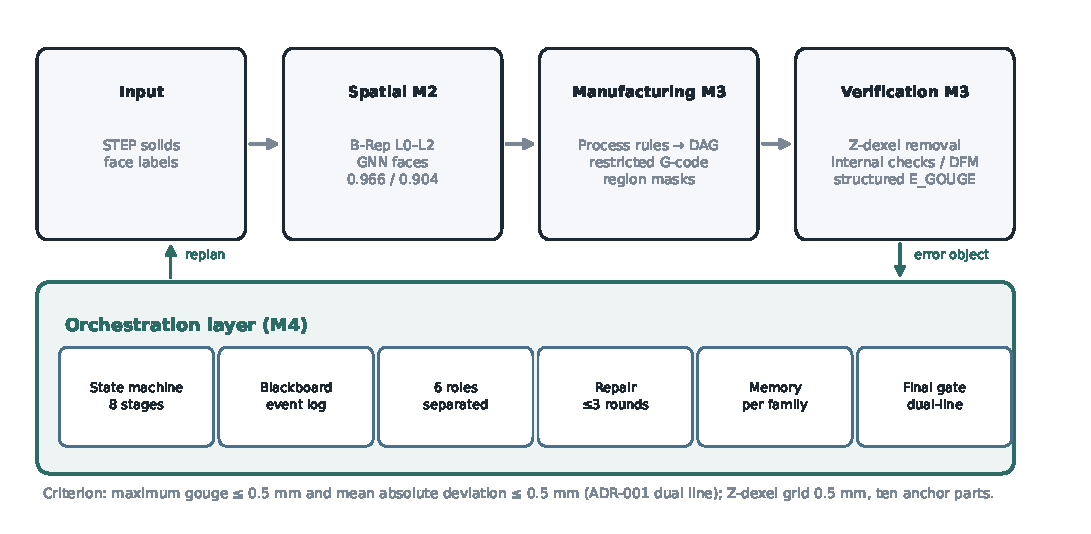
\includegraphics[width=\textwidth]{fig1.pdf}
  \caption{System overview. The upper path runs from part input through spatial and manufacturing modalities to verification; the lower path holds the state machine, blackboard, six roles, bounded repair and episodic memory. Arrows from verification back to planning carry structured errors with operation attribution. M2--M4 label the spatial, manufacturing and orchestration stages; L0--L2 are progressive boundary-representation digests; DFM denotes design-for-manufacture checks; E\_GOUGE is the structured gouge error.}
  \label{fig:1}
\end{figure}

\subsection{Spatial Modality: Boundary-Representation Digests and Face Labelling}

A part is compressed into three levels of digest before anything reaches a model. Level 0 holds global invariants: face, edge and concave-edge counts, bounding box, volume and surface area. Level 1 is a histogram of surface and feature types. Level 2 is a per-face table of surface type, area, normal and adjacency, served in pages so that context grows with the number of features rather than the number of faces.

Machining features are labelled by a three-layer message-passing network with 0.35 million parameters, taking face features, edge features (convexity, concavity, dihedral angle) and a type embedding, and producing one of 25 per-face labels. The model is trained on MFCAD++ \cite{Colligan2022}. Recognition is upstream of the contribution: its output only seeds the operation graph, and the final judgement is the simulated removal volume rather than classification accuracy.

\subsection{Manufacturing Modality: Process Envelope, Operation Graph and Restricted Programs}

The process library encodes material, cutter and parameter envelopes as clamping functions. Given a requested spindle speed, feed or depth of cut, the library returns the value clipped into the envelope together with an explicit violation record; it never silently rewrites the request. Planning produces a linear operation graph in the order face milling, pocketing, drilling and contouring. The stock leaves 1 mm above the finished top face, because with zero allowance the facing operation would have no material to remove and the simulation would degenerate into a no-op.

The emitter produces only whitelisted G and M codes (G0/G1/G2/G3, plane and compensation groups, canned drilling cycles, unit and feed modes). A parser reconstructs the program into a toolpath intermediate representation carrying operation labels, and performs three static checks: unknown codes, cutting with the spindle off, and rapid traverses through stock. Text and intermediate representation are checked against each other in both directions. This is the first layer of verifiability, and it is deliberately shallow: a syntactically perfect program can still cut the wrong region.

\subsection{Region-Masked Toolpath Generation}

Let $h(x,y)$ be the target height field obtained by rasterising the triangulated solid at grid resolution $r=0.5$ mm, and let $\rho$ be the cutter radius. For a target cutting layer $L$, define the material set and the feasible set of tool centres as

\begin{equation} \label{eq:mask}
M(L) = \{(x,y) \mid h(x,y) > L\}, \qquad
\mathcal{F}(L) = \Lambda_r \setminus \bigl( M(L) \oplus D_{\rho} \bigr),
\end{equation}

where $\Lambda_r$ is the grid of column centres and $D_{\rho}$ is the discrete disc used by the simulator. All sets and the dilation in Equation~\ref{eq:mask} are interpreted on this grid, not as an exact offset of the continuous solid. A permitted centre at layer $L$ cannot cover a represented target column above $L$ under that same disc. This establishes a discrete no-gouging invariant; it does not establish complete removal or safety between grid samples. Parallel passes descend through layers with axial depth $a_p$. Each emitted block carries a \texttt{HM<pass>\_L<level>} tag for operation attribution. Missing target columns and finite-cell boundary effects are evaluated separately with an independent cutter--triangle routine.

\subsection{Orchestration, Bounded Repair and Episodic Memory}

The state machine permits only the transitions \texttt{INIT}$\to$\texttt{ANALYZE}$\to$\texttt{PLAN}$\to$\texttt{EMIT}$\to$\texttt{VERIFY}, followed by \texttt{ACCEPT}, a \texttt{REPAIR}$\to$\texttt{EMIT}$\to$\texttt{VERIFY} loop, or \texttt{ESCALATE}. An illegal transition raises rather than being handled by convention. A blackboard is the only shared medium; every write and every decision enters an event log with role and sequence number, and a content fingerprint supports replay checks. Six roles -- analysis, planning, post-processing, verification, repair and final review -- read only upstream keys and write only their own. They do not call one another.

Repair has two fixed steps: a bounding-box plan, then the region-masked plan. If the second still fails, the run escalates with the blocking error object attached. Three rounds is a hard guardrail, not an observed convergence limit. Memory is indexed by part family, derived from the number of target height layers, and keyed by a failure signature of the form \emph{family}$|$\emph{error code} with no part identifier; only previously successful remedies are reused.

\subsection{Third-Party Verification Chains}

Two external kernels test different properties. CAMotics 1.2.0 \cite{CAMotics2020} simulates the same program, stock and cutters using a surface-mesh algorithm; we compare remaining workpiece volume. Volume agreement alone does not establish pointwise agreement or equal acceptance decisions. OpenCAMLib 2023.1.11 \cite{OpenCAMLib2023} uses continuous cutter--triangle intersection on a tessellated mesh, sampled along cutting paths at 0.5 mm spacing. For the toolpath audit, cutter diameters follow the actual operations, with radius reduced by a 0.02 mm tangency allowance. A separate geometry-reconstruction check uses a Ø0.02 mm point probe. Shrinking that probe tests artifacts in the reconstructed height field; it does not change or invalidate the finite-radius toolpath audit. Neither chain models machine dynamics or certifies unsampled motion.

A further chain checks the input geometry rather than the cutting algorithm. The ten STEP files are tessellated through FreeCAD's \texttt{Part.Shape.tessellate(0.05)}, written as binary STL and read by OpenCAMLib's \texttt{STLReader}, bypassing the JSON geometry cache that the verifier uses. This is an independent triangulation, serialisation and geometry-reading path. It is not a second boundary-representation kernel: STEP parsing still uses Open CASCADE. Agreement constrains discrepancies between these two mesh-construction paths on the tested parts; it does not rule out shared bias in Open CASCADE or establish agreement between two computer-aided design kernels.

\subsection{Datasets, Models and Reproducibility}

The anchor set is ten multi-level pocket parts from the RPTU Zenodo record 17035762 (CC BY 4.0), supplied with STEP files, reference programs and renderings \cite{RPTU2025}. Face labels for these parts were produced for this study: 206 faces in 62 feature instances, with two annotators agreeing at $\kappa=0.751$ (95\% confidence interval 0.570--0.912) on a stratified sample of 30 faces and complete agreement on the machined/unmachined binary decision. A rule-based pre-labelling pass matched only 54.4 percent of faces, which is why recognition was learned rather than scripted. The recognition network was trained on the 7,998/1,500/1,998 train/validation/test split of MFCAD++ for 40 epochs.

The external set was drawn from MFCAD (MIT licence, 15,488 STEP files). Filtering on the feature sequence in file names gave 1,947 mappable candidates; geometric filtering for 3--10 height layers and 8--60 faces left 130 parts, scaled by longest edge to 80 mm so that the Ø6 cutter and 0.5 mm thresholds still apply. These are synthetic regular solids with no bosses and mostly single-layer features. They show that the method does not depend on the ten anchor parts; they do not show that it handles arbitrary industrial geometry.

Simulation uses a 0.5 mm grid and cutter diameters from Ø1.5 to Ø10 mm chosen per operation. Fifteen language models were evaluated: five locally quantised Q4 models on a single RTX 4090 through Ollama, and ten cloud models accessed through a keyless service using account credit, with no self-provisioned API keys. The primary local model is Qwen3-8B (Q4\textunderscore K\textunderscore M, 8.2B) \cite{Qwen3_2025} at \texttt{temperature}=0 with thinking disabled. Cloud and local models share prompts and scoring. Offline scripts regenerate the result ledger and figures from stored outputs; separate revision scripts audit denominators and independently reconstruct work-order references. Regression tests cover both the original pipeline and these audits. Recomputing archived metrics is distinct from re-executing the model experiments.

\subsection{Independent Reference and Metric Audit}

The original work-order scorer constructs a reference by executing the expected calls through the same gateway as the model calls. A rejected feature can therefore disappear from both solids. In revision we independently construct the twenty easy-set targets from rectangular and cylindrical removal primitives, taking their Boolean union before subtracting it from the stock. This bypasses gateway preconditions and nominal-volume checks, while retaining the same Open CASCADE kernel. It tests reference-construction logic, not cross-kernel agreement.

The task generator stores some hole centres to one decimal place but prints integer coordinates in the instruction. We consequently distinguish a latent-specification target from a prompt-visible target built using the printed coordinates. The latter is the primary reference for assessing what the model could infer. Instructions are reconstructed from the retained generator and seed because original prompt bytes were not archived. Archived exported solids are read without rerunning models or executing generated scripts; hashes identify every input used in the audit. Agreement with the original reference is checked separately from agreement with each reconstructed target.

At the time of writing, the full-precision contract reconstruction is complete for all twenty tasks; the prompt-visible version has one unresolved task, and the script route has one unresolved task. Unresolved comparisons are reported as bounds over the remaining tasks, never as point estimates, and the thirty-item hard sets have not been reconstructed independently.

Export success means that the recorded run produced an artifact, not that every call committed. The archived \texttt{legal} count checks a known tool name and the presence of required arguments before commit; it is not a full-schema or postcondition acceptance rate. Semantic agreement is removed-volume IoU $\geq0.9$ against the explicitly named reference, not exact instruction satisfaction. The archive audit reports execution errors separately; where stored errors were truncated, their counts are lower bounds. The thirty-item and later task sets retain their original references and are not promoted to independently validated semantic benchmarks by the easy-set audit.

\subsection{Statistical Analysis}

No confirmatory hypothesis tests are performed. Part-level violation counts carry Wilson intervals; the paired plain-versus-guard comparison uses an exact McNemar test on discordant parts \cite{McNemar1947}, and threshold sensitivity is reported from 0.1 to 20 mm.  Wilson 95\% score intervals \cite{Wilson1927} accompany archived pass counts as nominal binomial summaries. Curated parts, geometry-based filtering and repeated stock variants violate a simple random-sample interpretation; these intervals are not population safety bounds. In revision, paired work-order differences are resampled by task, keeping both interface outputs together. These exploratory bootstrap intervals condition on the archived model responses and the stated reference construction. They do not estimate variation across fresh model calls, prompts or independent CAD kernels. Failed executions receive zero in all-task IoU means; conditional means use only executed outputs with recorded scores, and their denominators are reported separately. A missing measurement is not silently treated as a failed model output. Model-comparison scores are primarily single runs at \texttt{temperature}=0; one repeated cloud call returned 0.60 and then 1.00. No model ranking or effect of parameter count is established. External tool-centre samples within a part are correlated and are not independent trials.

\subsection{Human and Animal Research}

Three computer numerical control programmers each answered 30 binary questions about simulated outputs, and two annotators labelled the anchor parts. Participants were told how their responses would be used and took part voluntarily; no personal or health data were collected. \texttt{[AUTHORS: confirm the exact consent wording before submission.]} No animal experiments were performed. The human-study result is reported in Results and Discussion as a sanity check only, with the reason for that downgrade stated explicitly.

\section{RESULTS AND DISCUSSION}

We report the pipeline in the order it runs, then turn the verifier on itself. Pass counts are fractions; the intervals that belong to them appear with the acceptance-criterion results.

\subsection{Face-Level Machining Feature Recognition}

The three-layer message-passing network reaches 0.9660 accuracy and 0.9042 mean intersection over union on the MFCAD++ test split (Figure~\ref{fig:2}). Removing edge features yields 0.6969 and 0.4462 on the same held-out test split, supporting their usefulness in this recognition model. A decision tree records 0.9075 and 0.7198 on a different validation split; these historical values are reported for context, not as a matched test-set comparison or evidence of superiority. Recognition is an upstream component, not the principal contribution or a demonstration of foundation-model multimodal learning.

\begin{figure}[htbp]
  \centering
  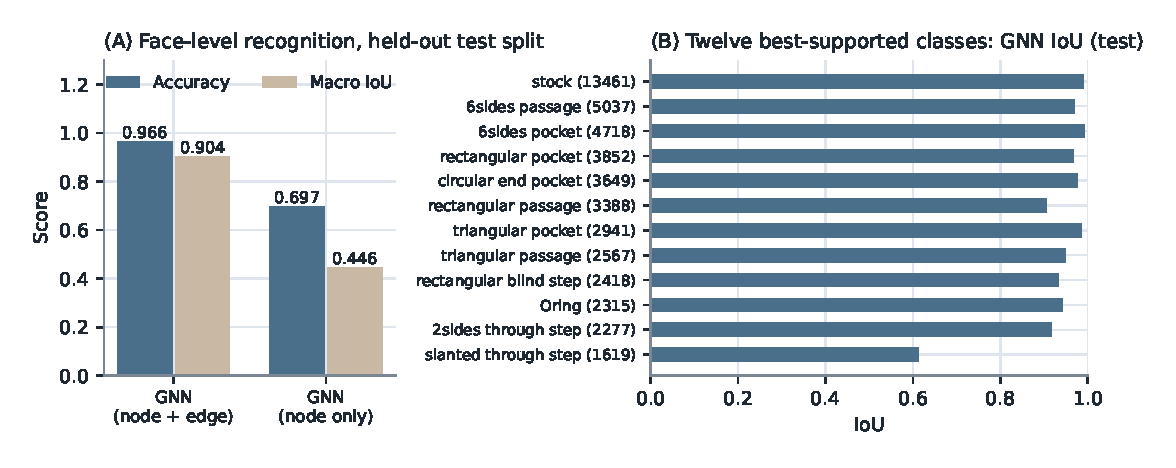
\includegraphics[width=\textwidth]{fig2.pdf}
  \caption{Face-level machining feature recognition. (A) Graph-network and node-only results on the same held-out test split. (B) Per-class intersection over union for the twelve best-supported classes under the full model, with test face counts in parentheses.}
  \label{fig:2}
\end{figure}

\subsection{Three Routes Compared on the Anchor Parts}

Table~\ref{tab:1} and Figure~\ref{fig:3} compare three ways of producing a program for the same ten parts, the same stock and the same cutters. A conventional face-milling route built from FreeCAD Path operators passes 2 of 10. A bounding-box plan produced by our own earlier generator passes 2 of 10. The region-masked generator passes 10 of 10, with zero total gouging and a worst mean deviation of 0.206 mm.

\begin{table}[htbp]\small
\caption{Three toolpath routes on the ten anchor parts. Gouge volume is summed across parts; mean absolute deviation is reported for the worst part. Passes use Equation~\ref{eq:accept}.}
\centering
\begin{tabular}{lccc}
\toprule
Route & Total gouge (mm$^3$) & Worst mean deviation (mm) & Dual-line pass \\
\midrule
FreeCAD Path operators & 215,126.7 & 12.225 & 2/10 \\
Bounding-box plan & 196,726.7 & 12.118 & 2/10 \\
Region-masked plan & 0.0 & 0.206 & 10/10 \\
\bottomrule
\end{tabular}
\label{tab:1}
\end{table}

\begin{figure}[htbp]
  \centering
  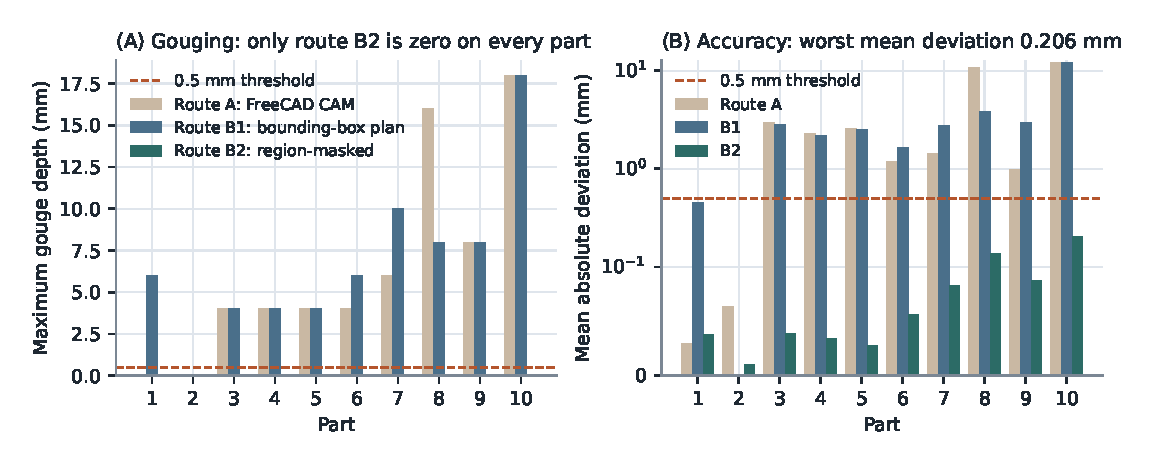
\includegraphics[width=\textwidth]{fig3.pdf}
  \caption{Three toolpath routes on the ten anchor parts. (A) Maximum gouge depth and (B) mean absolute deviation; dashed lines mark the 0.5 mm threshold. Gouging under the region-masked route is identically zero within the discrete representation.}
  \label{fig:3}
\end{figure}

The failure of the conventional route is a semantic one, and we report it as a negative result. Its face-milling operator is defined to machine flat to a given height; when several disconnected regions share that height, the toolpath degenerates to the bounding box of all of them. Four boundary configurations were tried and none constrained the traversal. This says that a general-purpose facing operator does not match layer-by-layer machining on multi-level pockets. It does not say that the underlying computer-aided manufacturing package is incapable of machining these parts with a full process setup.

Switching off the radius inflation in Equation~\ref{eq:mask}, with everything else unchanged, takes the dual-line result from 10/10 to 0/10 and produces a worst gouge of 18.000 mm. Without inflation, a tool centre can approach a step while the cutter overlaps the higher plateau; the resulting vertical gouge depends on the local height difference, not on adding a horizontal cutter radius to that height. The internal zero-gouging result does not come from knowing which regions to keep. It comes from dilating those regions by the cutter radius before placing any tool centre.

\subsection{Failure of a Single Maximum-Deviation Criterion}

A single $\max|S-P|$ does not distinguish excess removal from residual stock (Figure~\ref{fig:4}). Our dual-line criterion makes that distinction, at the cost of accepting some large local residuals; this choice is not a replacement for a part-specific dimensional tolerance. Four observations support Equation~\ref{eq:accept}. First, the worst 10 mm deviation under the region-masked route is entirely residual: maximum gouge depth is 0.000 mm on all ten parts, and every column above threshold has material higher than the target, which a finishing pass can remove. Second, the same toolpath's maximum deviation is an artefact of resolution: coarsening the grid from 0.5 to 1.0 mm changes the worst deviation on parts 1, 8 and 10 from 6, 8 and 10 mm to 0, 0 and 0 mm, simply because the narrow columns disappear. Third, on the worst part, 2.844 percent of columns exceed 0.5 mm and all of them lie within one cell of a step boundary; they form a single connected cluster. This is a cutter that cannot reach, not a path that wandered. Fourth, adding a 0.75 mm finishing cutter drives mean deviation to zero, but the program grows from 10,439 to 28,245 lines. This is a sensitivity example under the discrete model, not a proof of attainable physical accuracy or a proposed production process.

\begin{figure}[htbp]
  \centering
  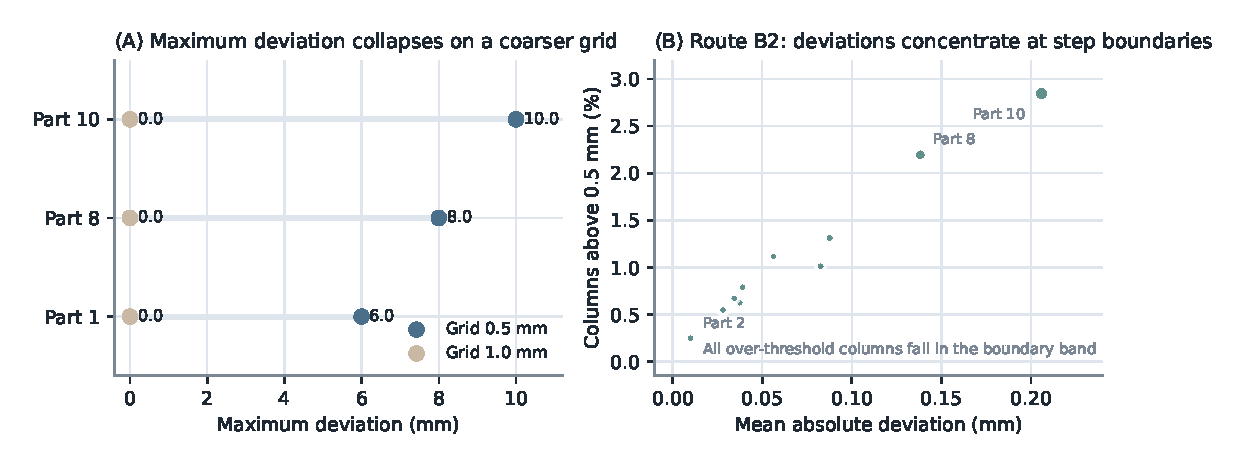
\includegraphics[width=\textwidth]{fig4.pdf}
  \caption{Behaviour of the acceptance criterion. (A) Maximum deviation of an identical toolpath under two grid resolutions; the coarser grid collapses the maximum to zero. (B) Fraction of columns above threshold and mean deviation for the region-masked route; marker area shows residual volume.}
  \label{fig:4}
\end{figure}

\begin{table}[htbp]\small
\caption{Wilson 95\% score intervals for every pass count cited in the main claims. Counts are reported as $k/n$ rather than percentages; the Wald interval degenerates at proportions of 0 and 1.}
\centering
\begin{tabular}{lccc}
\toprule
Result & $k/n$ & Point estimate & Wilson 95\% interval \\
\midrule
Region-masked dual-line pass & 10/10 & 1.000 & [0.7225, 1.0000] \\
FreeCAD operator route & 2/10 & 0.200 & [0.0567, 0.5098] \\
No-inflation baseline & 0/10 & 0.000 & [0.0000, 0.2775] \\
End-to-end without / with repair & 2/20, 20/20 & 0.100, 1.000 & [0.0279, 0.3010], [0.8389, 1.0000] \\
Third-party generated toolpath & 9/10 & 0.900 & [0.5958, 0.9821] \\
External set dual-line pass & 130/130 & 1.000 & [0.9713, 1.0000] \\
\bottomrule
\end{tabular}
\label{tab:2}
\end{table}

Table~\ref{tab:2} gives nominal score intervals under an independent Bernoulli sampling model. The anchor set is curated, the external set is geometrically filtered, and the twenty orchestration tasks reuse ten designs. These intervals therefore do not establish industrial-population reliability, and the two stock variants must not be interpreted as twenty independent designs. The external set expands geometric coverage; it does not convert the internal criterion into an externally validated safety guarantee.

\subsection{Orchestration and Bounded Repair}

Twenty tasks were formed from the ten parts at two stock allowances (1.0 and 2.5 mm), with part family derived from the number of target height layers (Figure~\ref{fig:5}). With repair disabled, 2 of 20 pass. With repair enabled and cold memory, 20 of 20 pass at a mean 0.90 repair rounds. With warm memory, 20 of 20 pass at 0.15 rounds, and 17 of 20 are accepted on the first attempt rather than 2. Split by family, the unrepaired bounding-box plan passes 0.500 of parts with at most two layers and 0.000 of parts with three or more; the more layers there are, the less a single bounding box resembles the part.

\begin{figure}[htbp]
  \centering
  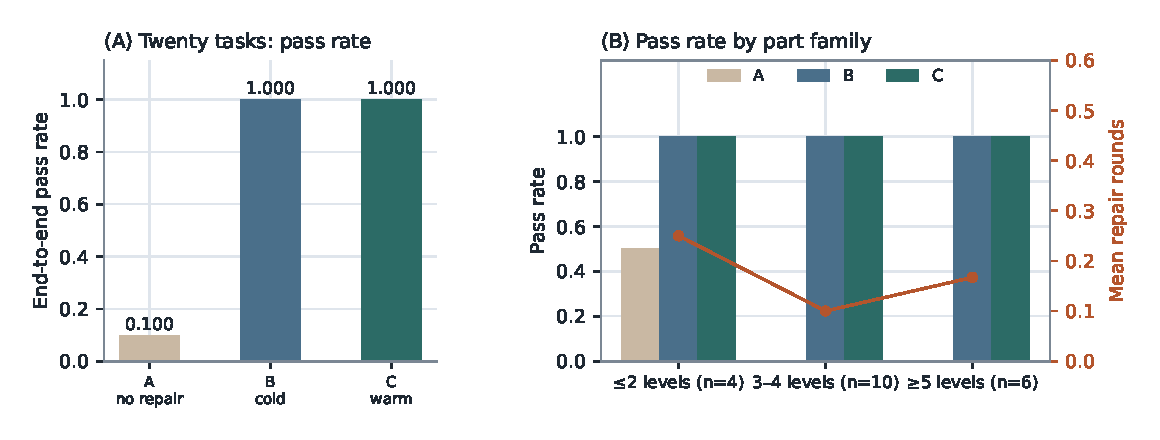
\includegraphics[width=\textwidth]{fig5.pdf}
  \caption{Orchestration ablation over twenty tasks. (A) End-to-end pass rate with repair disabled, with cold memory and with warm memory. (B) Pass rate by part family; the line shows mean repair rounds for the warm-start group.}
  \label{fig:5}
\end{figure}

The 20/20 describes recovery within a constructed suite, not general agent capability. The final repair option is a region-masked plan already known to pass these anchor designs; zero internal gouging alone would not guarantee the residual-error condition on another design. The 2/20 without repair and the drop from 0.90 to 0.15 rounds describe the cost of starting from a poor plan and reusing remedies. The six roles were deterministic strategies at this stage. The twenty tasks reuse ten geometries, and warm memory is evaluated within this constructed sequence, not on a held-out family split.

\subsection{Fifteen Models at the Decision Points}

Two semantic choices were handed to Qwen3-8B: planning strategy (bounding box or height map) and repair action (switch or escalate). Geometry and verification stayed deterministic. Table~\ref{tab:3} collects the action-space comparison that frames the paper.

\begin{table}[htbp]\small
\caption{Archived work-order comparison for Qwen3-8B. Exports are not semantic successes. Agreement means removed-volume IoU $\geq0.9$ against the original contract-generated reference. All-task means include failed exports as zero. These references are audited separately below.}
\centering
\begin{tabular}{llccc}
\toprule
Interface & Set & Exports & Agreement & All-task IoU \\
\midrule
Contract & Easy & 20/20 & 20/20 & 0.985 \\
Script & Easy & 19/20 & 2/20 & 0.165 \\
Contract, run 1 & Hard & 30/30 & 22/30 & 0.789 \\
Contract, run 2 & Hard & 30/30 & 22/30 & 0.769 \\
Script, run 1 & Hard & 26/30 & 2/30 & 0.099 \\
\bottomrule
\end{tabular}
\label{tab:3}
\end{table}

Under a neutral prompt the model chose the conservative height-map strategy 20/20 times and ignored cycle time. Rewriting one sentence to state that every hundred program lines cost about thirty seconds flipped all twenty decisions to the aggressive strategy, including parts with ten layers that necessarily gouged. No conditional behaviour by layer count appeared; the model followed the most salient instruction, not the geometry. Eighteen of twenty runs in that group gouged on the first attempt, up to 18 mm, and were rescued only by bounded repair. The verifier, not the model, decided whether the repaired outcome was acceptable. Choosing the masked strategy was not free: the mean of twenty per-task program-length ratios is 11.37. Total line counts are 59,788 versus 4,682; the mean ratio is not the ratio of these totals. The cycle-time statement was a prompt heuristic, not a measured machining-time model. Archived calls used about 350 tokens and 0.15--0.25 s per call.

Structured errors did not improve model repair. Three feedback conditions -- structured fields, prose, and no numeric values -- produced identical pass rates, identical repair-round distributions and identical action choices, while the structured version spent 79 percent more prompt tokens. With only two repair options and an obvious answer, the model had no use for the numbers. We therefore make no claim that structured errors improve language-model repair; we claim they let the \emph{program} locate the offending operation, which is what the deterministic repairer consumes.

The original easy-set archive records exports on 20/20 contract tasks and 19/20 script tasks. Its conditional mean removed-volume IoUs are 0.985 and 0.174; counting the failed script as zero changes the latter all-task mean to 0.165. These scores are agreement with the archived reference, not independent proof of correctly following each order. Thirteen contract tasks contain recorded execution errors, with 19 error entries in total, even though all twenty meet the original IoU threshold. The executor continues after a rejected call, and the original reference uses that same executor. Agreement can therefore reward a feature omitted from both outputs.

The independent reconstruction is only partly complete. For the contract route it rescores all twenty tasks against a full-precision target: mean removed-volume IoU is 0.7526, and 9 of 20 reach 0.9. The gap from the archived 0.985 is expected: the reconstructed target includes cutters that the gateway had rejected, so it credits material the archived reference also omitted. The prompt-visible target gives 0.7871 over the 19 tasks that can be scored; NL07 remains unresolved because its rounded reference produces Boolean cells that fail the volume identities. The script route is bounded rather than estimated: NL03 shares the stock's outer shell, so OCC returns the stock unchanged from \texttt{stock.cut(output)} while \texttt{output.cut(stock)} returns the output, and no comparison satisfies the volume identities. With failed exports counted as zero and the unresolved tasks left null, the script mean lies between 0.1788 and 0.2288 against the full-precision target and between 0.1811 and 0.2811 against the visible target. These are bounds, not point estimates. The reconstruction uses the same Open CASCADE kernel; it validates reference-construction logic, not cross-kernel agreement.

Table~\ref{tab:3} also reports the retained thirty-item hard-set runs rather than the earlier eight-item pilot, whose complete per-item report is no longer available. Those hard-set scores remain conditional on the original reference construction. Removed-volume scoring is still important: in a retained corner-placement example, whole-solid IoU is 0.933 while removed-volume IoU is zero. It avoids dilution by unchanged stock, but cannot correct a defective reference.

The fifteen-model contract study uses thirty orders and a common interface template. Fourteen models export 30/30 outputs; Llama-3.1-8B exports 29/30 because one response fails JSON parsing. The recorded legality metric is 1.000 over emitted calls for every available model, but it counts known tool names and required-argument presence before execution. A failed response contributes no calls to that denominator, and rejected commits need not reduce it. It therefore establishes neither perfect syntax across responses nor semantic correctness. Conditional removed-volume IoU against the archived reference spans 0.462--1.000, with the best local mean 0.842; six cloud models meet the archived geometric criterion on all thirty orders. One additional endpoint returns HTTP 400 for all thirty requests and is reported separately as unavailable, not as a model-capability failure. Parameter counts do not isolate a scale effect: model families, training and quantisation differ, and cloud counts are undisclosed.

One item exposed an ambiguity in the task set. The original wording specified two pockets symmetric about a line without stating their distance from it; eight of nine models produced other defensible layouts. Adding the missing distances and rerunning only that item took the ten cloud models from 1 correct to 10/10 at intersection over union 1.0, while all five local models still failed. A benchmark has to be shown unambiguous before it can be used to rank models, and this episode also sets a boundary on the contract: all fifteen models had perfect legality, and not one asked for the missing distance.

A second, harder set of twenty orders targeted only the weaknesses that data had exposed -- compound depths, implicit constraints and negation chains -- with every item made uniquely solvable. It widened the cloud--local gap from 0.158 to 0.239 and cut the number of error-free cloud models from six to three, but did not fully separate the frontier models. Where errors remain is more informative than the score: cloud models fail almost exclusively on jointly satisfying several spatial constraints, and barely fail at arithmetic; local models show the opposite pattern. Adding a genuinely different geometry did not add difficulty. A sloping-bottom pocket, implemented with a new contract operation, was solved 6/6 by nine of ten cloud models and by three of five local models, including the two smallest local models that scored worst elsewhere. The parameter names are literal and the order states the numbers directly. Difficulty came from how much had to be inferred, not from how complex the feature was. The extension cost thirty lines in the geometry worker, one schema entry and one precondition; the height field, the removal simulator and the evaluation pipeline were untouched.

When requirements were deliberately incomplete, the correct behaviour was to ask. Five under-specified orders were given two permitted outputs, a set of calls or a clarification. Cloud models hit 3.1 of 4 strong ambiguities and local models 0.8 of 4; human scoring of clarification quality on a 0--2 scale gave cloud models 6.8 of 8 against 0.8 of 8 locally. Two observations complicate ranking by a single score. A cloud model with 0.973 on the hard set hit only 1 of 4 clarifications, while a local model with 0.412 hit 2 of 4 -- the best local result. A model that never asks will confidently machine an ambiguous drawing, so a ranking built only on intersection over union is not a ranking of shop-floor safety. We also learned that ``depth 1'' was read as 1 mm by all fifteen models: an engineering default is not an ambiguity, and a test that treats it as one records correct behaviour as an error.

Bounded multi-round repair solved 9 of 10 harder orders within two rounds, but two feedback forms again gave identical per-task outcomes and differed only in prompt tokens. A controlled probe on the one item that resisted repair -- ``upper-left corner'' read as centre -- fixed the wrong plan and varied only the feedback, three times each. Vague feedback succeeded 0/3; structured feedback naming leftover material succeeded 0/3; structured feedback that supplied the correct coordinates succeeded 3/3. This probe does not establish that feedback can never repair misunderstanding; it shows failure under the evaluated model, item and feedback budgets. Our deterministic repairer works because it receives operation identifiers and face identifiers, not a sentence saying something is wrong.

Asked to write machine instructions directly, with the stock, feature extents, target heights and allowed code set all supplied, the model passed 0/10. Eight of the ten programs were whitelist-legal, yet none was geometrically correct; the deepest cut reached 48 mm. Free-form modelling scripts ran on 3 of 5 parts and met a 5 percent volume tolerance on 1 of 5, failing for semantic reasons such as constructing a compound instead of a Boolean difference. The problem is not whether the model can write code. It is whether the code knows that material has to be removed.

An offline diagnostic raises the endpoints of the ten archived programs to the nearest target-column height, without adding passes or changing horizontal coordinates. It still gives 0/10: mean worst gouge falls from 10.596 to 4.996 mm, while mean residual volume rises from 25,503 to 25,623 mm$^3$. This operation does not compute clearance for the full cutter footprint or the interior of every segment, and is therefore neither a safe projection nor an upper bound on repair. It demonstrates only that this particular endpoint-lifting heuristic does not rescue the programs. An iterative model or planner allowed to add coverage was not evaluated.

These results motivate restricting what the deployed model may emit while retaining independent checks on the resulting geometry. Free-form programs are not intrinsically unjudgeable: they can be executed in an appropriate sandbox and checked geometrically. The present results concern the tested implementations and prompts, not an impossibility of repairing free-form outputs.

\subsection{Auditing the Verifier Itself}

Ten anchor parts and a self-written simulator invite two questions, so we addressed both with code that does not share our algorithms (Figure~\ref{fig:6}, Table~\ref{tab:4}). The external set of 130 parts passes the same dual-line criterion 130/130, with worst gouge 0.000 mm and worst mean deviation 0.306 mm; every height-layer group from 3 to 10 passes fully.

\begin{table}[htbp]\small
\caption{Third-party audit of the acceptance criterion. Percentages are fractions of sampled tool-centre positions judged by continuous cutter--triangle intersection.}
\centering
\begin{tabular}{lcc}
\toprule
Measure & Ten anchor parts & 130 external parts \\
\midrule
Third-party gouge under region-masked plan & 0.76\% (2,822/371,230) & 3.275\% (316,398/9,660,095) \\
Third-party gouge without inflation & 10.59\% (43,260/408,646) & 14.468\% (1,571,946/10,865,228) \\
Our dual-line pass, region-masked & 10/10 & 130/130 \\
With half-cell guard, gouge count & 41 & 5,167 \\
With half-cell guard, dual-line pass & 9/10 & 107/130 \\
With half-cell guard, residual volume & 3.4$\times$ & 4.42$\times$ \\
Parts with any flag, plain / guarded & -- & 128/130, 19/130 \\
Parts with deep flag, plain / guarded & -- & 94/130, 8/130 \\
Worst cutter depth (mm), plain / guarded & -- & 71.104, 42.288 \\
\bottomrule
\end{tabular}
\label{tab:4}
\end{table}

CAMotics simulates the same programs, stock and cutters and reports the remaining workpiece volume; across ten parts the mean relative difference from our remaining-volume figure is 1.15 percent (maximum 3.22, 95th percentile 2.90). Because the stock is identical, this is also an aggregate statement about removed volume, but it does not establish pointwise agreement or equal acceptance decisions; the difference grows with the number of layers because step boundaries get longer. OpenCAMLib answers a question CAMotics cannot: whether an individual tool-centre position contacts material in continuous geometry. Its point-cutter height field agrees with our rasterisation on at least 99.828 percent of 256,000 columns at 1.0000 coverage intersection over union, with 120 columns differing at curved step edges. It rejects the no-inflation baseline at 10.59 percent of positions while flagging only 0.76 percent under the region-masked plan, and it produces none of those flags for toolpaths it generates itself. Our criterion accepts 9/10 of those third-party toolpaths; part 10 fails the accuracy line at 0.538 mm with genuine residual material and zero gouging. A verifier that rejects a bad route and accepts an independently produced good one is not simply rubber-stamping its own generator.

An independent geometry chain speaks to the input mesh. Tessellating the STEP files through FreeCAD into binary STL and reading them with OpenCAMLib, bypassing our JSON cache, reproduces the height field to at least 99.984 percent column-wise. Four purely planar parts differ by 0.0000 mm; the six parts with curved faces differ on 15 columns total (at most 0.06 percent) by one layer depth, because two tessellators cut arcs differently. Gouge counts change from 2,822/43,260 to 2,826/43,262, under 0.15 percent. STEP parsing still uses Open CASCADE, so this is an independent triangulation, serialisation and geometry-reading path, not a second boundary-representation kernel.

The audit also found a blind spot that we would not otherwise have seen, and we report it rather than smoothing it away. Radius inflation measures distance from column centre to column centre, whereas continuous geometry measures from column centre to step edge; near an arc the discrete mask can under-cover by half a cell, and the generator and verifier share the disc that hides it. Three observations identify this as a resolution artefact. Refining the grid on one part from 0.5 through 0.25 to 0.125 mm reduces the third-party gouge rate monotonically from 1.332 to 0.432 to 0.143 percent. Adding a half-cell guard to the inflation radius cuts gouge positions from 2,822 to 41. But the guard has a real cost: residual volume rises from 4,606 to 15,886 mm$^3$, and the dual-line result falls from 10/10 to 9/10. Thus this tested guard does not achieve both objectives on the evaluated set. This is not an impossibility result for other paths, cutters or continuous-offset constructions.

The external set exposes a more serious disagreement. Grid coverage averages 96.849 percent and falls to 77.465 percent. A finite-radius cutter may touch a neighbouring plateau even when its centre lies in a column omitted from the target mask; that interaction is absent from the internal check. Column-centre dilation also misses contact at slanted boundaries. The finite-cutter oracle flags 316,398 sampled positions, including 77,363 deeper than 0.5 mm, with a maximum predicted depth of 71.104 mm. These are not uniformly shallow violations.

A revision audit aggregates by part rather than treating millions of correlated path samples as independent trials. The unguarded plan has at least one flag on 128/130 parts and a violation deeper than 0.5 mm on 94/130 (Wilson 95\% CI 0.64--0.79). With a half-cell guard those counts fall to 19/130 and 8/130 (0.03--0.12), but the maximum finite-cutter depth remains 42.288 mm. Equal-weight mean per-part flag rates are 3.1973 percent and 0.0384 percent, respectively; pooled-point rates are 3.2753 percent and 0.0558 percent. The guard never moves a part from non-violating to violating: 86 parts improve, none worsen, eight remain above the line and 36 stay below it (exact McNemar $p<10^{-25}$). The count is not a knife-edge threshold effect: it is 102/130 at 0.25 mm, 94/130 from 0.5 to 5 mm, 87/130 at 10 mm and 49/130 at 20 mm; the guarded count is 13/130 at 0.25 mm, 8/130 at 0.5 mm and 6/130 from 0.75 mm upward. Violations concentrate where mask coverage is low: 34/36 parts below 96\% coverage exceed 0.5 mm, against 28/32 at 96--99\% and 32/62 at 99\% or above (Spearman $\rho=-0.42$ for coverage against the binary violation indicator). This association is consistent with the coverage mechanism; it does not establish coverage as the only cause. The guard reduces exposure, but does not eliminate the external safety failures.

Point-probe sensitivity is a different measurement. Shrinking the geometry probe from Ø0.02 to Ø0.002 mm reduces discrepant columns from 199 to 2; a Ø0.0002 mm probe leaves one. This explains sensitivity in pointwise mesh reconstruction, not the finite-radius toolpath violations. The value 71.104 mm occurs in both fields of the archive. It cannot be dismissed as a point-probe artifact in the toolpath audit, which uses operation-specific cutters. All these depths are predictions on a tessellated model, not measurements of physical cutting.

Accordingly, zero gouging is restricted to the internal single-valued height-field representation and shared discrete disc. Passing that criterion does not establish continuous-mesh safety: the external oracle disagrees on most unguarded parts. The disagreement is a measured limitation of the proposed generator--verifier pair, not a safety issue resolved merely by disclosing it.

\begin{figure}[htbp]
  \centering
  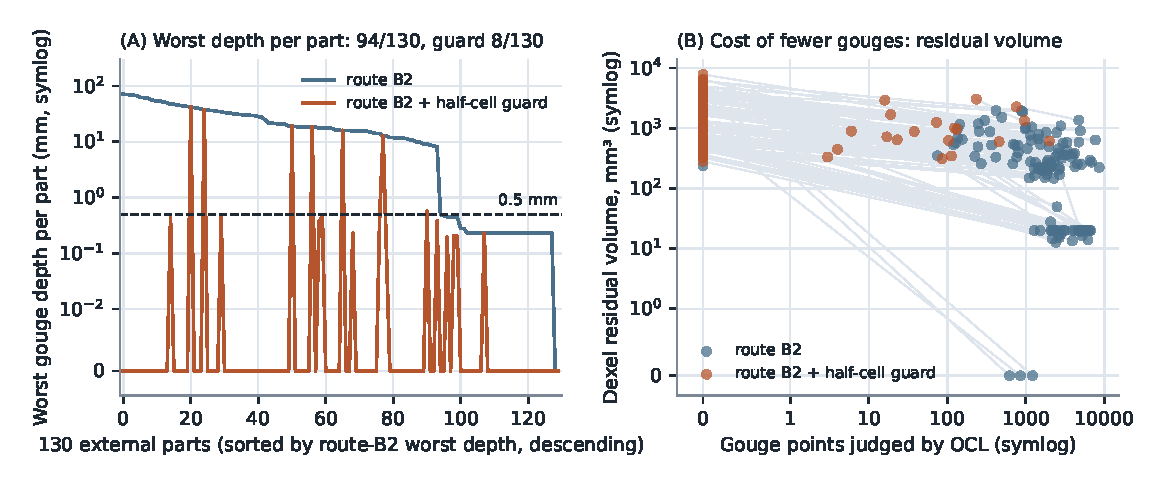
\includegraphics[width=\textwidth]{fig6.pdf}
  \caption{Third-party criterion over 130 external parts with operation-specific cutters. (A) Worst predicted gouge depth per part for the plain mask and with the half-cell guard, sorted by the plain-mask depth; the dashed line is 0.5 mm. (B) Per-part shift from the plain to the guarded mask: fewer judged gouge points, more residual volume. Both axes use symlog scaling so that exact zeros remain visible rather than being replaced by a display floor.}
  \label{fig:6}
\end{figure}

\subsection{Verifier Self-Check and Human Agreement}

On the anchor set the verifier processes 65 operations, 2,271 program lines and 1,797 parsed segments, with whitelist checks passing 10/10. Injected gouging, residual material and interference are each detected 10/10; a clean program raises no false interference alarm. Nine error objects carry operation identifiers, face identifiers and per-operation attribution, and six design-for-manufacture warnings (fillet radii below cutter radius, and similar) are reported without being used to judge acceptance.

Three computer numerical control programmers answered 30 binary questions each and agreed with the verifier at $\kappa=1.000$. We downgrade this to a sanity check. The visualisation legend fixed red to gouging and the question was exactly ``is there gouging?'', so a trivial classifier that counts red pixels also scores 1.0000. The experiment shows only that the alarms and the pictures do not contradict each other; it is not evidence of independent human judgement. A construct-validity study would need an information channel decoupled from the simulator output, such as giving readers the toolpath and the drawing without the heat map.

\section{CONCLUSION}

Tool-mediated grounding requires checking the engineering state, not just the model's response. Our design-and-manufacturing testbed separates valid calls, executable outputs and agreement with the requested removal. The twenty-work-order comparison favours the implemented contract interface over free-form scripts, but different prompts and output budgets prevent attributing that difference to action space alone. The fifteen-model study measures language-understanding variation within one interface, not a causal effect of model scale. Direct numerical control generation on ten anchor parts is a separate failure diagnostic.

The deterministic pipeline supplies an explicit division of responsibility. Region masks restrict tool-centre positions; a dual-line criterion separates excess removal from average residual error; bounded repair replaces failed operations. On two stock variants of ten designs, repair changes internal acceptance from 2/20 to 20/20, and warm memory changes mean repair rounds from 0.90 to 0.15. These results describe recovery on a constructed suite with a known successful fallback, not general-purpose agent planning or industrial reliability.

Negative results delimit these observations. The tested facing operator does not implement the required layer-aware semantics, which is not a verdict on the full manufacturing package. Feedback formats produce identical outcomes in a restricted repair task, and endpoint lifting does not rescue archived direct programs. These probes do not establish that richer feedback or replanning cannot work.

The strongest methodological lesson is that the evaluator must also be checked. CAMotics provides an aggregate-volume cross-check, whereas OpenCAMLib exposes finite-cutter violations missed by the internal grid model. Although 130/130 external parts pass internally, 94/130 have an externally predicted violation deeper than 0.5 mm. A half-cell guard reduces that count to 8/130 and never turned a non-violating part into a violating one (86 improved, none worsened), but it multiplies residual volume by 4.42 and lowers internal acceptance to 107/130. This is evidence of an unresolved safety--accuracy tradeoff for the tested generator, not a proof that other constructions cannot satisfy both. Point-probe sensitivity does not dismiss the finite-cutter failures. The discrete no-gouging invariant remains valid only within the shared representation.

Transfer is limited by curated and synthetic geometry, a single-valued height field and simulation-only evaluation. The external parts are scaled to an 80 mm longest edge; undercuts, five-axis motion and physical effects such as deflection are not represented. The human study is a sanity check because its colour legend reveals the answer. Model comparisons primarily use single responses, incomplete prompt archives and references generated through the same contract machinery; only the twenty easy orders receive the independent reference reconstruction reported here, and that reconstruction is itself partial. Two tasks could not be scored under one or both reference definitions because Boolean operations on coincident shells did not satisfy the volume identities, so the script result is a bound rather than a point estimate. The thirty-item hard sets have no independent reconstruction and remain provisional evidence of semantic fidelity. Reusing Open CASCADE in the reconstruction separates reference-construction logic, not geometry kernels. No new multimodal encoder is trained, and no general multimodal intelligence or deployment readiness is claimed.

The next controlled evaluation should freeze prompt-visible targets independently of the executor, preserve complete requests and outputs, and compare matched information and inference budgets across repeated runs. Manufacturing deployment additionally requires resolving the finite-cutter failures and testing effects absent from simulation. The present contribution is a reproducible way to expose shared errors across language, geometry and manufacturing interfaces, rather than a claim that a closed interface alone makes those errors disappear.

\section*{Acknowledgments}

\subsection*{General}

[AUTHORS: add any non-author contributions here, with permission. Remove this bracketed line if there are none.]

Language models were used as experimental subjects and as research assistants. Fifteen evaluated models produced tool calls, programs and clarification responses to supplied work orders; the archives retain scored outputs and metadata, but not every original response or prompt. AI assistance also supported manuscript drafting, code development, experimental audit design and numerical analysis during revision. The offline audits did not make new inference calls to the evaluated models. [AUTHORS: specify the AI assistants and versions used, verify the extent of assistance across the project, and confirm review of the code, analyses and final text before submission.] Human authors remain responsible for the validity, interpretation and presentation of the work. No AI tool is listed as an author.

\subsection*{Author Contributions}

[AUTHORS: replace with initials and full surnames, e.g. ``X. Zhang conceived the study and designed the experiments. Y. Li implemented the gateway and ran the evaluations. All authors wrote and approved the manuscript.'']

\subsection*{Funding}

[AUTHORS: replace with the full name of each supporting body, the awardee and grant numbers in square brackets, or state that no funding was received. Example of the required no-funding sentence: ``The authors acknowledge that they did not receive funding for this work.'']

\subsection*{Conflicts of Interest}

The authors declare that there is no conflict of interest regarding the publication of this article. Cloud-model experiments were run against a keyless service using account credit; no provider supplied funding, data, computational resources beyond ordinary paid access, or editorial input.

\subsection*{Data Availability}

The ten anchor parts come from the RPTU Zenodo record 17035762 \cite{RPTU2025} and are redistributed under CC BY 4.0 with the original attribution retained. The face-level annotations produced for those parts, all generated programs, all result files, the Wilson interval implementation, the six figure scripts and the complete reproduction script are available in the project repository at \texttt{https://github.com/Lobot777/cadcam} (archived as \texttt{https://doi.org/10.5281/zenodo.24361565}).

Two third-party datasets are \emph{not} distributed with this repository. MFCAD++ \cite{Colligan2022} is supplied by Queen's University Belfast under CC BY (dataset DOI 10.17034/d1fec5a0-8c10-4630-b02e-b92dc81df823); after downloading it from the publisher's page, \texttt{scripts/extract\_mfcad.py} reproduces the 7,998/1,500/1,998 split used here. The 130-part external set was derived from the MFCAD corpus released under the MIT licence and must be obtained from its upstream distributor; the selection and scaling script is provided, but the source STEP files are not. The full upstream corpora are not bundled; their licences and attribution conditions remain applicable when readers obtain them. Omission from this repository should not be read as a prohibition on redistribution under those licences.

Re-running the geometric, toolpath, orchestration and third-party-audit experiments requires no model server once their data and software dependencies are installed. The revision audits preserve the original archives and identify inputs by SHA256; independent reference reconstruction requires FreeCAD. Re-running model comparisons requires the specified weights or cloud access. The archives retain partial responses, generated artifacts and per-task measurements, not a complete immutable record of every prompt, response and model revision. In particular, one ambiguous item was replaced after rewording and some working output paths were reused. This limits exact replay and retrospective independent rescoring.


\printbibliography

\end{document}
